\chapter{Layered Editor Architectures}
\label{chap:layeredArchs}
{\em *** Version: \today~ ***}



\bc
* fix gesture to edit Rendering, unless gesture becomes something special
* rendering or presentation? Rendering is more clear, but editing the rendering does not make sense. (maybe just explain)

HOE HEEFT PRE HIERMEE TE MAKEN? pre geeft geen berekening, maar alleen verband, dus zelfs als level i opgeleverd door pre, dan nog is het invoer

- Numbering 0 = doc, downwards like lines on a page.
** ?Add a $lower = EDIT~levels~gesture$ condition that states the result is what we mean with the gesture?



IMPORTANT there seems to be an invariant that for a j:  i>j, all mappings are correct 
  ..           ...       
 .  .    ..   .   .   .. 
.    ....  ...     ...  .
 no it's not asymmetric. find out more about this.
 maybe it's just that a level is never presented twice without intr, and vice versa

RENDERER IS SPECIAL, LOWER THING IS NOT A TREE, EXPLAIN THAT THIS CHAPTER ONLY HOLDS FOR HIGHER LAYERS


\ec
MAYBE DO SOME NON layered stuff first? to explain what spec. will mean.


% intro

prev. chap. spec for layer but not edit and transform

Next chapter, we give Haskell for the combination

\section{Spec}

First by figures, then give spec.


?? Add arrow for intended gesture update?

\subsection{Connecting layers}

figure with in and out from prev. (hiding internal)

\begin{figure}\begin{small}\begin{center}\begin{center}
\epsfig{file=pics/eps/singleToMulti.eps, width=125mm}\end{center}
\caption{Blaa}\label{singleToMulti} 
\end{center}\end{small}\end{figure}

Now connect

need to remove one update: plaatje 3 layers, one layer

\begin{figure}\begin{small}\begin{center}\begin{center}
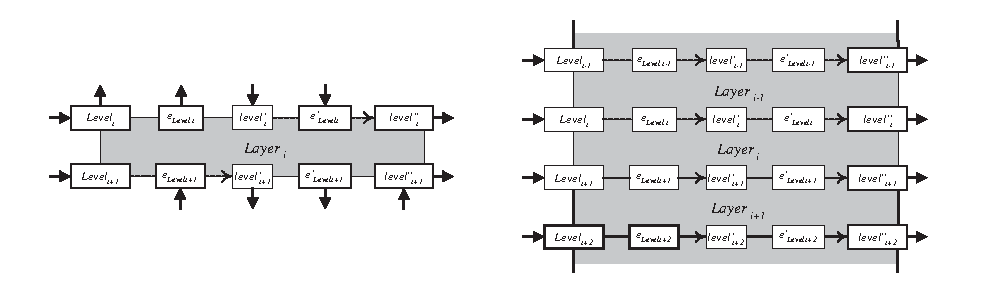
\epsfig{file=pics/eps/connectingLayers.eps, width=125mm}\end{center}
\caption{Blaa}\label{connectingLayers} 
\end{center}\end{small}\end{figure}



need something on top id
need something at bottom display and receive gesture. Also explain that user does not give e rendering

gesture depends on level, not edit. Also on other levels?


\begin{figure}\begin{small}\begin{center}\begin{center}
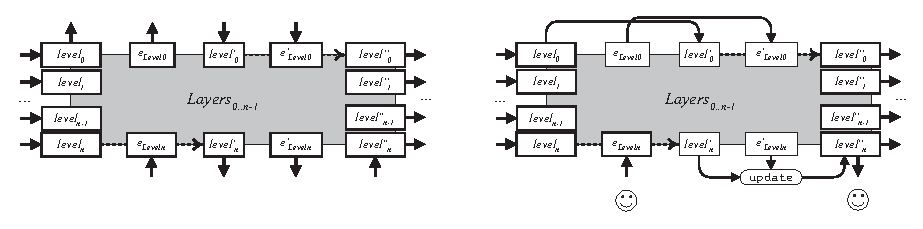
\epsfig{file=pics/eps/topAndBottom.eps, width=125mm}\end{center}
\caption{Blaa}\label{topAndBottom} 
\end{center}\end{small}\end{figure}


\subsection{Specifying connected layers}

First try: add i and leave out Edit and Transform

\begin{small}\( \begin{array}{lcl}  \label{inv:incrementality}
{\tt interpret_i}  ::  Sheet_{Intr,i} \rightarrow Level_{i+1} \rightarrow Level_{i} \rightarrow  Edit_{Level_{i+1}} \rightarrow Edit_{Core_{i}\times Info\idwn_{i}} \\
{\tt present_i}  ::  Sheet_{Pres,i} \rightarrow Level_{i} \rightarrow Level_{i+1}  \rightarrow Edit_{Level_{i}} \rightarrow Edit_{Core_{i+1}\times Info\iup_{i+1}}\\
\\
\end{array}\) \\
\( \begin{array}{rcll}  
level_{i+1} 	& = & Present_{i}~level_{i}						& \text{\{Precondition\}}\\
\\
level'_{i+1} 	& = & {\tt update}~e_{Level_{i+1}}~level_{i+1}                 & \text{\{Compute intermediate lower level\}}\\
e_{Core_{i} \times Info\idwn_{i}}  & = & {\tt interpret}_{i}~sheet_{Intr,i}~level_{i+1}~level_{i}~e_{Level_{i+1}} & \text{\{Compute higher core update\}}\\
e_{Level_{i}} & = & {\tt reuse}_{Intr,i}~level_{i}~e_{Core_{i}\times Info\idwn_{i}}     & \text{\{Reuse extra state\}}\\
level'_{i} & = & {\tt update}~e_{Level_{i}}~level_{i}                 & \text{\{Compute intermediate higher level\}}\\
\\\
level'_{i} & = & Interpret_{i}~level'_{i+1}						& \text{\{Intermediate condition\}}\\
\\
level''_{i} & = & {\tt update}~e'_{Level_{i}}~level'_{i}                 & \text{\{Compute final higher level\}}\\
e'_{Core_{i+1}\times Info\iup_{i+1}}  & = & {\tt present}_{i}~sheet_{Pres,i}~level'_{i}~level'_{i+1}~e'{Level_{i}} & \text{\{Compute new lower core\}}\\
e'_{Level_{i+1}} & = & {\tt reuse}_{Pres,i}~level_{i+1}~e'_{Core_{i+1}\times Info\iup_{i+1}} & \text{\{Reuse extra state\}}\\
level''_{i+1} & = & {\tt update}~e_{Level_{i+1}}~level_{i+1}                 & \text{\{Compute final lower level\}}\\
\\
level''_{i+1} & = & Present_{i}~level''_{i}						& \text{\{Postcondition\}}\\
\end{array}\)
\end{small}
\begin{center}(First try)\end{center}\vspace{1em}


level updates are double., so leave out one. intr leave out higher \{Compute intermediate higher level\} and pres leave out lower \{Compute final lower level\}. End up with:

\begin{small}\( \begin{array}{lcll} 
level'_{i+1} 	& = & {\tt update}~e_{Level_{i+1}}~level_{i+1}                 & \text{\{Compute intermediate lower level\}}\\
level''_{i} & = & {\tt update}~e'_{Level_{i}}~level'_{i}                 & \text{\{Compute final higher level\}}\\
\end{array}\)
\end{small}

Now we don't have computations for $level'_0$ and $level''{n}$. $e_n$ is not defined and $e'_0$


On top level, put the edit op back in, and just copy the not updated level:

\begin{small}\( \begin{array}{lcll} 
e'_{Level_{0}}  = e_{Level{0}}\\
level'_{0} =  level_{0}\\
\end{array}\)
\end{small}

On the bottom level, edit op comes from user. 

\begin{small}\( \begin{array}{lcll} 
e_{Level_{n}}  = EditGesture ??\\
level''_{n}  =  {\tt update}~e'_{Level_{n}}~level'_{n}\\
\end{array}\)
\end{small}


If we remove the double updates, and add the top and bottom stuff, we get a final specification:

\begin{itemize}
\item subscripts cannot be dropped anymore. Use data defs from prev chap (multiple layer perspective)
\item levels and layers mismatch, j and i
\item present, interpret, Sheet, all get i.  level,core,info h is level... i and level.. L is level.. i+1
\item update is generic, so no subscripts
\item only need one update on each layer, choose the source level because of inc comp. (ref to previous chap)
\item Edit and Transform disappear
\end{itemize}

Given level0..n for which Pres holds and an edit gesture, compute level''0..n so Pres holds again.

\begin{small}\( \begin{array}{lcl}  \label{inv:incrementality}
\text{\bf type}~Level_{0}  =  Core_{Intr,0} \times Extra_{Intr,0} \times Info\idwn_{0} \\
\text{\bf type}~Level_{n}  =  Core_{Pres,n} \times Extra_{Pres,n} \times  Info\iup_{n}\\
\lefteqn{\forall j:1 \le i \le n-1:}  \\
\text{\bf type}~Level_{j} =  Core_{Pres,j} \times Extra_{Pres,j}  \times Info\iup_{j}   
                                       =  Core_{Intr,j} \times Extra_{Intr,j} \times Info\idwn_{j}\\

e_{Level_{n}}  = EditGesture ??\\
e'_{Level_{0}}  = e_{Level{0}}\\
level'_{0} =  level_{0}\\
level''_{n}  =  {\tt update}~e'_{Level_{n}}~level'_{n}\\
\lefteqn{\forall i:0 \le i \le n-1:}  \\
{\tt interpret_i}  ::  Sheet_{Intr,i} \rightarrow Level_{i+1} \rightarrow Level_{i} \rightarrow  Edit_{Level_{i+1}} \rightarrow Edit_{Core_{i}\times Info\idwn_{i}} \\
{\tt present_i}  ::  Sheet_{Pres,i} \rightarrow Level_{i} \rightarrow Level_{i+1}  \rightarrow Edit_{Level_{i}} \rightarrow Edit_{Core_{i+1}\times Info\iup_{i+1}}\\
\\
\end{array}\) \\
\( \begin{array}{rcll}  
level_{i+1} 	& = & Present_{i}~level_{i}						& \text{\{Precondition\}}\\
\\
level'_{i+1} 	& = & {\tt update}~e_{Level_{i+1}}~level_{i+1}                 & \text{\{Compute intermediate lower level\}}\\
e_{Core_{i} \times Info\idwn_{i}}  & = & {\tt interpret}_{i}~sheet_{Intr,i}~level_{i+1}~level_{i}~e_{Level_{i+1}} & \text{\{Compute higher core update\}}\\
e_{Level_{i}} & = & {\tt reuse}_{Intr,i}~level_{i}~e_{Core_{i}\times Info\idwn_{i}}     & \text{\{Reuse extra state\}}\\
\\\
level'_{i} & = & Interpret_{i}~level'_{i+1}						& \text{\{Intermediate condition\}}\\
\\
level''_{i} & = & {\tt update}~e'_{Level_{i}}~level'_{i}                 & \text{\{Compute final higher level\}}\\
e'_{Core_{i+1}\times Info\iup_{i+1}}  & = & {\tt present}_{i}~sheet_{Pres,i}~level'_{i}~level'_{i+1}~e'{Level_{i}} & \text{\{Compute new lower core\}}\\
e'_{Level_{i+1}} & = & {\tt reuse}_{Pres,i}~level_{i+1}~e'_{Core_{i+1}\times Info\iup_{i+1}} & \text{\{Reuse extra state\}}\\
\\
level''_{i+1} & = & Present_{i}~level''_{i}						& \text{\{Postcondition\}}\\
\end{array}\)
\end{small}
\begin{center}(Final specification)\end{center}\vspace{1em}

\begin{itemize}
\item Starting the editor
\item level'' is level for next edit step
\item level for first needs to be initialized
\end{itemize}



%																
%																
%																
\section{}
\begin{itemize}
\item edit ops starting higher + es safety
\item tricky. maybe need to point out diff between skipping and processing
\end{itemize}

\section{}
\begin{itemize}
\item skipping cycles + es safety
\item ref to edit model
\end{itemize}

\section{Conclusions}







